% 三、拟采取的研究方案及可行性分析。
% 研究设计按2026-09-20用户要求明确参数与工作量；2026-09-21补齐复核汇总和随机对照规则。
\subsection{研究方法与技术路线}
本课题先核验数据与误差，再以同骨干四组检验约束区域及替代解释；检测器冻结后，用校准与排序分析残留错误。主检验解释误报与小变化召回的权衡，辅助检验评价这些错误能否被复核发现。

\textbf{数据与误差路线（图\ref{fig:mct-route-diagnosis}）。}核对影像、标签及矿区来源，复现基线并抽查错误，形成质量清单、固定划分与机制实验样本。

\textbf{区域约束路线（图\ref{fig:mct-route-constraint}）。}开展同骨干区域比较、强度匹配及DonaNet区域替换，以误报与小变化召回判定权衡；在验证集选定检测器后冻结。

\textbf{复核评价路线（图\ref{fig:mct-route-reliability}）。}独立拟合温度并冻结排序，比较同面积下的剩余错误，追踪不同约束改变的错误类型及其可复核性。

配准或标签歧义主导误差时先处理质量问题；无改善时保留对照。外部验证与人员复核在核心实验后有条件开展。

以下列出主检验、辅助检验和条件探索各自的比较对象及判断依据。
\begin{center}
\begin{tabular}{p{0.14\linewidth}p{0.28\linewidth}p{0.39\linewidth}}
\hline
任务 & 首要比较 & 支持条件与解释范围 \\
\hline
主检验 & 同骨干背景约束对全图约束 & 误报改善且小变化召回非劣；随机、强度、平滑及阈值对照排查替代解释。 \\
辅助检验 & 固定检测器的组合排序对最强单指标 & 同预算及同实际面积核对下，剩余误报与漏检均改善；仅解释离线纠错上限。 \\
条件探索 & 外观分层、掩码污染及近邻局部替换 & 报告效应差和反例，不以总体收益、单层显著或梯度现象单独证明机制。 \\
\hline
\end{tabular}
\end{center}
\textbf{（1）数据验收与独立划分。}
先下载并校验MineNetCD正式归档，登记版本、许可证、文件校验值、矿区ID及场景来源；检查影像与标签配对、有效像素和配准质量。重复或无效样本按事先固定的规则处理，保留剔除原因；不得依据模型测试表现删除困难矿区。沿用原论文60/10/30矿区分组，主机制实验固定为50个训练矿区、10个独立校准矿区、原10个验证矿区与原30个测试矿区。训练与校准部分复用预实验已保存的50个训练和10个保留矿区名单，在正式归档核验后登记；所有主比较方法均在相同的50个训练矿区重新训练。

误差诊断和规则设计限于训练、验证矿区。采用MineNetCD发布的ResNet-18孪生基线，固定解码器及输入通道，以DonaNet为近邻方法；官方60/10/30完整协议仅在核心实验后补充复现，结果单列。

正式训练输入为$256\times256$像素，统一运行60轮；每轮每个训练矿区最多抽取200对影像，总计不超过10000对，轮间轮换样本，样本较少的矿区使用全部可用影像。同种子下各组共用抽样顺序与增强序列；校准、验证和测试采用各自矿区全部有效裁块。开发期最多进行12次、每次15轮的短训练，正式配置按验证矿区宏平均F1选择并冻结；主检测概率阈值固定为0.5。四组区域对照各运行3个种子，共12次完整训练；DonaNet原法和局部区域替换各3次，共6次；另预留最多6次完整训练，优先用于主方法及DonaNet的强度敏感性配置各3次。额外方法、外部数据或官方完整协议的训练均占用这6次额度，按开发阶段需要取舍，不另行叠加，完整训练总量不超过24次。平滑、概率校准与窗口排序均复用已保存的预测或模型，不额外训练检测器。

训练集拟合模型，验证集选择方法及排序，校准集只拟合温度，测试在规则冻结后评估。每个模型、每个种子只拟合一次温度，不随验证反馈重拟；测试标签不参与选择。归一化、增强及预训练权重的矿区覆盖均纳入审计。官方权重复现与主协议重训单列，不把60矿区训练结果直接与50矿区结果比较；适应或微调另记可见信息范围。

\begin{center}
\begin{minipage}{\linewidth}
  \centering
  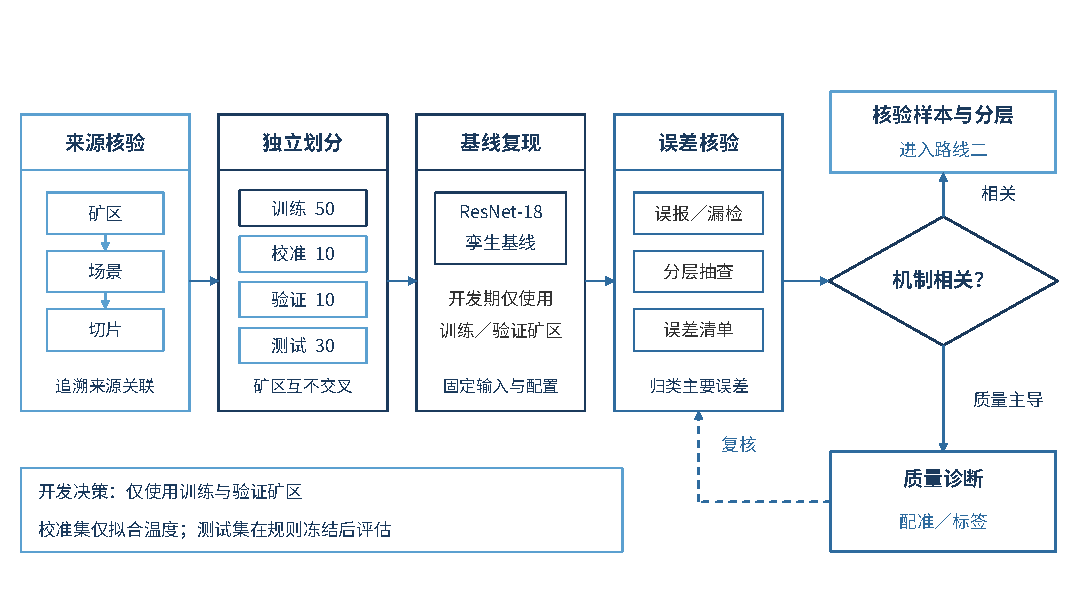
\includegraphics[width=\linewidth,trim=0 0 0 12mm,clip]{figures/vector/F03_route_diagnosis.pdf}
  \captionsetup{justification=justified,singlelinecheck=false}
  \captionof{figure}{研究路线一：核验矿区、场景及切片来源，复现基线并诊断误差；配准或标签歧义主导时，先处理质量问题，再确定机制实验样本及分层。}
  \label{fig:mct-route-diagnosis}
\end{minipage}
\end{center}

% 避免小标题及其首段仅一行留在图后页尾。
\begingroup\clubpenalty=10000
\textbf{（2）背景限定约束与可归因对照。}
给定两期影像$x^{(1)},x^{(2)}$及训练变化标签$Y$，固定取共享ResNet-18第二残差阶段的特征（步长8）。在输入网格将$Y=0$的有效区经$3\times3$腐蚀一次，再按$8\times8$格投影；仅腐蚀后格内均为1时置$M_i=1$，不插值。256像素输入对应$32\times32$特征网格，全图有效掩码按格内全部有效规则投影。令$f^{(t)}_i$为该层特征，$\bar f^{(t)}_i$为通道单位化形式，构建
\par\endgroup
\begin{equation}
\mathcal{L}_{\mathrm{bg}}=\frac{\sum_i M_i\|\bar f_i^{(1)}-\bar f_i^{(2)}\|_2^2}{\max(1,\sum_i M_i)},\qquad
\mathcal{L}=\mathcal{L}_{\mathrm{seg}}+\lambda\mathcal{L}_{\mathrm{bg}}.
\end{equation}
分割监督$\mathcal{L}_{\mathrm{seg}}$覆盖全部有效像素；空掩码的约束为零，单位化稳定项为$10^{-6}$。网格内未变化不保证整个感受野无变化，固定模型诊断另按距变化边界的距离汇总，不把腐蚀视为感受野隔离。掩码只由训练标签生成，测试前向不读取真值。权重在$\{0.05,0.10,0.20\}$中选择，三组共用候选及短训练预算，以其验证表现均值选共同权重，再开展三种子比较。

四组分别为无一致性、全图一致性、背景限定一致性和等面积随机一致性，约束损失按实际特征格数归一化。随机组在$32\times32$网格上枚举七种非恒等旋转或镜像，对完全落在共同有效区且不同于$M$的候选去重后均匀抽取。以零容差保持面积、形状及到最近裁块外边界的无符号距离分布，不匹配真实变化边界；无候选时回退$M$，不删样本或停用背景组约束。记录回退、重叠和输入变化像素覆盖率；区域差异不足时，不以无差异否定机制。抽样规则在训练前固定。

同一分割结果另作同等调参预算的平滑对照。强度诊断固定无约束短训练模型与训练样本，在共同编码器参数上计算约束梯度相对分割梯度的范数，以全图为参照，从$\{0.25,0.5,1,2,4\}$选背景权重乘数，使中位强度比最接近参照，随后冻结。开发匹配相对残差须不超过10\%，正式训练另报各轮差异；不匹配时只解释区域与强度共同效应。最多6次补充训练先保障主骨干三种子匹配，再用于DonaNet，外部及额外模型后置。

固定模型诊断在同一影像对内配对变化格与未变化格；变化格要求输入格全部有效且为变化像素，混合格不进入此项诊断。保持格数，将变化格比例设为0、25\%和50\%，每档抽样10次。共用样本和权重，在同一编码器参数上计算梯度夹角，零范数记NA；另报损失、特征距离和输入变化比例，不更新参数或解释为训练收益。候选不足时各档共同退出并报告，该诊断不代表不足一格的小变化。DonaNet替换保留原图与风格化影像对输出间的Kullback--Leibler（KL）散度，仅改为同分辨率未变化区平均；KL方向、网络、增强、监督及预算不变。预测空间与主方案分开报告，无法复现时记录原因。

加入仅作用于经核验未变化区的颜色或亮度扰动，构成同一样本的受控敏感性对照。合成扰动不能代替自然矿区分布变化，故只有其结果与自然外观差异分层方向相符时，才讨论共同支持的条件性解释。配准偏移及明显标签争议样本独立标记，不把这些误差笼统归为域差异。

自然外观差异采用可复核的代理量。共同RGB波段沿用预实验的固定$[0,1]$归一化后取通道均值；每对影像在$3\times3$邻域腐蚀一次后的标注未变化有效区，计算两期灰度绝对差的中位数，再对矿区内影像对取中位数，得到$D_s$。分档界点固定为50个训练矿区中有效$D_s$的第50百分位数；偶数个有效矿区时取排序后居中两值的平均值。等于界点归入低档，高于界点归入高档，实际界点由训练数据计算并在测试前冻结。无有效未变化像素的影像对记为不适用，整矿区无有效对时不分层并报告数量；无有效训练矿区时停止该项探索。该量只用于预定分层，不参与模型推理、复核排序或测试调参；测试标签仅在冻结后用于评分和分层。

前期分析发现$D_s$与矿区变化像素占比同向共变，故各档同时报告误差与变化占比。自然分层统一解释为描述性条件关联，以背景误报率为主要依据，不用变化IoU归因于外观差异；机制解释依赖受控对照。配准争议样本分别纳入和排除，检验结果敏感性。$D_s$不单独区分光照、季节或地物因素，也不表示地质环境风险。

\textbf{（3）评价指标与假说判据。}
基础检测指标为变化类交并比（IoU）、F1分数、精确率和召回率，主报告矿区宏平均及分布。记误报、漏检和真负像素数分别为FP、FN和TN，背景误报率定义为$\mathrm{FP}/(\mathrm{FP}+\mathrm{TN})$。正式小变化定义为面积不超过训练集完整8连通变化分量第25百分位数的分量；仅统计不接裁块边界的完整分量，按最近秩法取排序后第$\lceil0.25N\rceil$个面积值，$N$为有效训练分量数。$N=0$时不定义面积阈值，该端点记为不可估计，仅保留总体误差分析。该定义表示本数据中的相对小变化，阈值在查看测试标签前登记；有可靠空间分辨率时同时换算地面面积。逐分量计算像素召回，在矿区内对分量等权平均，再对有效矿区等权汇总。预实验的64像素定义与既有NA结果保持原样，正式方案另行验证。

无变化矿区的变化IoU、F1、总体召回和漏检率记为不适用（NA）；无小变化矿区的小变化召回、无背景矿区的背景误报率及无正预测时的精确率同样记NA，不补零或满分。联合判据要求两个端点各有至少20个有效测试矿区、小变化累计至少100个完整分量；不足时仅作描述性解释，不放宽面积界点。每项指标列明有效矿区数和分母，该门槛不代表已获得充分统计功效。

设背景组相对同骨干全图组的矿区宏平均背景误报率差为$\Delta_{\mathrm{FP}}$，小变化召回差为$\Delta_R$。预设误报改善界$\epsilon=0.01$、召回非劣界$\delta=0.01$，均为绝对1个百分点，不是相对变化1\%。支持联合收益须同时满足$\Delta_{\mathrm{FP}}$的95\%区间上界低于$-0.01$，且$\Delta_R$的95\%区间下界高于$-0.01$。这是本研究事先选定的保守比较尺度，不作为已确认的业务容忍度，也不承诺实验必然达到；已有预实验中的总体召回下降不能因该阈值而改写为非劣。另报告完整效应区间及召回零损失界下的结果，“差异不显著”不能代替非劣证据。随机或平滑对照解释了主要收益时，不支持区域选择的机制解释；区间过宽时结论为证据不足；出现明确召回损伤时，报告该条件下的反例。

同时完整报告背景组相对无约束组的两端点效应，区分两种约束的相对差异与新增检测收益。利用保存概率补报精确率—召回率曲线；以验证集无约束组在0.5下的矿区宏平均召回为参照，在$\{0.01,0.02,\ldots,0.99\}$中为各组冻结最接近该召回的阈值，并列取较大者。测试时报告误报及实际召回差，不在测试集调阈值或声称严格等召回。若优势仅见于0.5工作点，则不解释为可分性改善；这些分析不增加训练。

各主配置固定采用17、29、43三个随机种子，同种子跨方法配对。先在每个矿区内平均不同种子及重复掩码的效应，再按矿区配对自助重采样估计区间，重采样时保留区内全部运行记录；重复掩码也不计为独立样本。区间解释限于本训练运行条件下的矿区变异；种子波动另行展示，不将像素、切片或每次训练运行计作新的独立矿区。区间固定为95\%双侧百分位区间，进行10000次矿区配对自助重采样，统计随机种子为1729，按各指标固定的有效矿区集合成对重采样。首要比较为同骨干背景组对全图组；随机和平滑为机制排除对照。误报优效与召回非劣按交并判据联合解释；多个额外确认性对照采用Holm校正并报告原始效应区间，剂量趋势、分层与扩展分析标为探索性。

总体联合判据针对全体适用矿区；高低外观分层及组间效应差均完整报告为探索结果，不事后挑选子集。梯度与性能分别解释：低剂量非单调不足以反驳机制，只有操纵有效且区间排除预设有意义效应时，才反驳相应剂量命题。

现有预实验不足以估计正式小变化端点的功效。数据验收后报告有效矿区数与可检测效应范围；区间过宽或端点不可估计时，保留权衡、失败条件及复现记录，负结果同样纳入研究。

\begin{center}
\begin{minipage}{\linewidth}
  \centering
  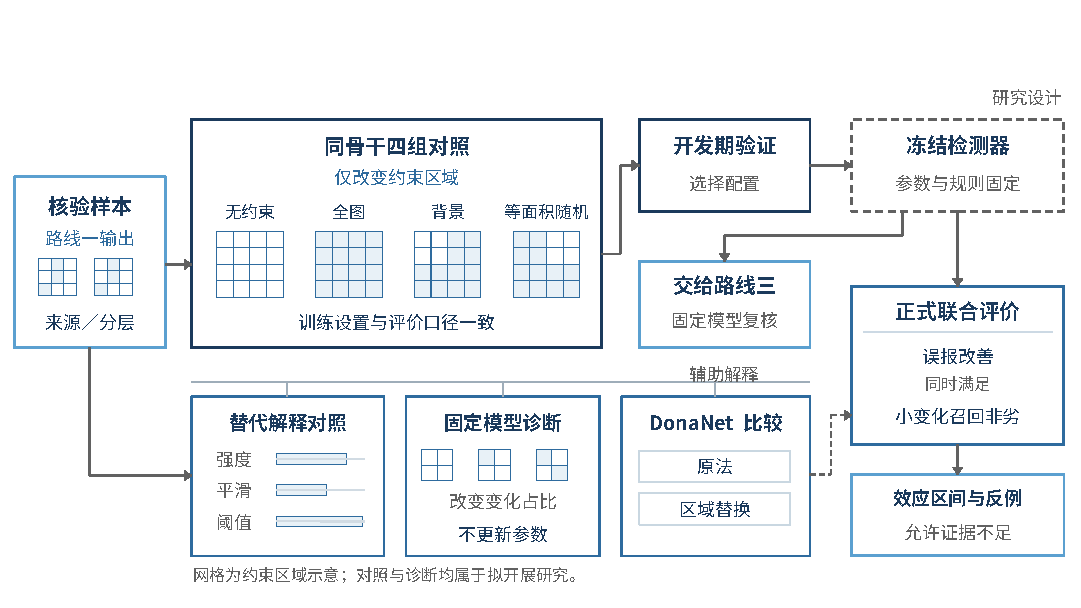
\includegraphics[width=\linewidth,trim=0 0 0 12mm,clip]{figures/vector/F04_route_constraint.pdf}
  \captionsetup{justification=justified,singlelinecheck=false}
  \captionof{figure}{研究路线二：约束区域与负迁移条件检验。四组依次为无一致性、全区域、背景位置与等面积随机约束；以误报改善和小变化召回非劣联合检验收益。图中对照与流程均为研究设计示意，不是测量结果。}
  \label{fig:mct-route-constraint}
\end{minipage}
\end{center}

\textbf{（4）校准、错误排序与复核效用。}
模型冻结后，仅用原图、水平翻转、垂直翻转和旋转180度四个可逆视图，不更新参数或归一化统计。各视图输出除以正温度$T$，转为概率后对齐取平均；独立校准矿区先区内平均对数损失、再矿区等权拟合$T$。Brier分数和15等宽区间的校准误差均先区内计算再宏平均，另报类别可靠性曲线。区分原图概率$p$与四视图概率$q$；$q$的校准改善不等于原图判决置信度改善，排序仍共用$p\geq0.5$的冻结预测。

将全图有效区域划为$64\times64$不重叠窗口，预测未变化区也参与排序。四视图的平均概率用于计算熵，概率方差用于计算分歧；原始熵取$T=1$，校准熵与分歧使用拟合的$T$。窗口内得分取像素均值，再按验证窗口的经验分位数将熵与分歧映射到$[0,1]$，以$S=\alpha H+(1-\alpha)V$组合，$\alpha\in\{0.25,0.50,0.75\}$。在10\%复核预算下，将剩余误报率、漏检率分别在其固定有效验证矿区中等权平均，再将两均值相加，以和最小选择组合权重及最强单指标。各候选共用同一端点集合；任一集合为空则不选择权重或最强单指标，按预设$\alpha=0.50$与各单指标逐项描述有效结果。若无有效验证窗口则停止排序评价。并列时权重按0.50、0.25、0.75，单指标按原始熵、校准熵、分歧排序；映射与选择均在测试前冻结。

“全图”为验收后固定的评测区域；有坐标时去除重叠位置，无坐标时仅为发布裁块集合的像素预算，不换算地理面积。连通分量先在原标签确定，去重后不完整者不计小变化端点并报数，不把残片另算分量。各矿区按有效面积比例取整窗，首个超预算窗即停止；同分按冻结的样本ID和行列排序。边缘窗只计有效像素，记录实际比例及余额。主预算10\%，补充0、5\%、20\%和完整曲线；随机排序重复20次。

同一预算上限下的实际面积可能不同。各矿区取各排序实际选中面积的最小值，沿既定窗口及窗内行列顺序截取等量有效像素，重算剩余错误。主预算与等实际面积的结论一致，才支持排序收益。末窗截取仅作离线敏感性分析，不推断人工整窗复核效率。

离线评估将选中窗口的预测替换为真值，剩余FP、FN仍分别除以复核前全图背景、变化面积。零分母记NA；有效矿区由真值与有效区域一次确定，各排序和预算共用并用于配对推断。另报真实变化覆盖、未选中区漏检；高置信度漏检预定义为真变化且原图$p\leq0.1$，仅作描述，不用于排序调参。

联合选择可计算时，以验证集最强单指标为对照；主预算下，两项矿区配对误差差值的区间上界均小于零，才支持同时改善。端点不可估计时不作联合结论，仅点估计降低作描述，单项改善说明取舍，零基线只报绝对差。该分析为辅助探索；真值替换仅估计理想上限，真实复核另记错误、耗时及一致性。

\begin{center}
\begin{minipage}{\linewidth}
  \centering
  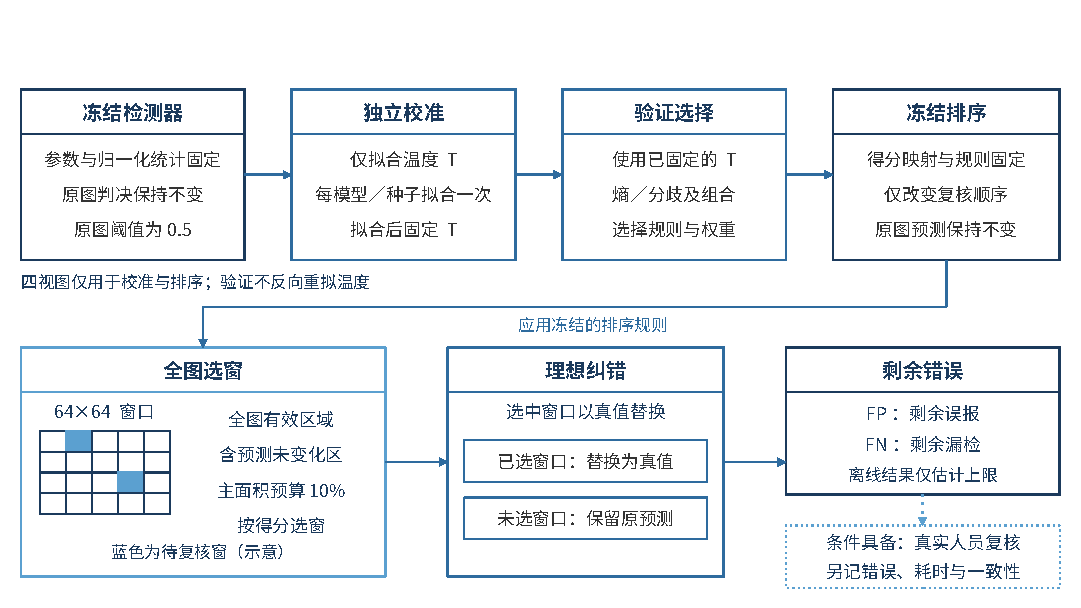
\includegraphics[width=\linewidth,trim=0 0 0 12mm,clip]{figures/vector/F05_route_reliability.pdf}
  \captionsetup{justification=justified,singlelinecheck=false}
  \captionof{figure}{研究路线三：校准、错误排序与固定面积复核。独立校准矿区只拟合温度，验证矿区选择排序规则；全图窗口进入候选集合。流程与窗口为示意，真值替换仅评价理想纠错上限，真实复核另需实施。}
  \label{fig:mct-route-reliability}
\end{minipage}
\end{center}

主复核采用验证集选定的检测器；另复用无约束、全图和背景组，按同一规则各自校准、冻结排序，追踪新增、消失及残留错误。排序收益在模型内比较，模型间仅描述错误及可复核性差异，不推断协同增益，不追加训练。

\textbf{（5）外部验证与矿山语义。}
核心实验后视资源开展EuroMineNet矿区隔离验证，对齐年度足迹与双时相任务的标签、波段、分辨率和时相，单列目标域可见信息。全球铜矿数据仅核对案例属性，不外推全部有色金属矿。专业解释以合作落实为条件；缺少影像或现场证据时，不把连通域解释为采矿事件。

\subsection{关键技术}
关键是核验来源与隔离数据用途，控制约束区域、强度及工作点，依据全图误报、漏检和覆盖判断检测与排序各自的收益。

\subsection{可行性分析}
采用单张现有A40，先按300个单卡GPU小时排期，非专属配额。验收后计时正式骨干与DonaNet各3轮，含读盘、验证及复核推理估算总量。超量先取消外部及额外模型，保障主比较与强度对照；仍不足则在测试前统一调整预算，保留三种子和相同条件。强度未匹配时只解释联合效应。
